\chapter{Measurement and analysis}

\section{Preparatory measurements}

Before the actual measurement can be understaken, a couple of preparations must be made such as setting the PMT voltages, the discriminator thresholds and finally testing the electronics with simulated pulses.

\subsection{Setting the counter}

The discriminator's rectangular pulse widths are set to \SI{50}{\nano\second}, this provides long enough pulses for the coincidences while also minimizing the amount of random coincidences which arise from the overlap of two successive pulses due to their finite width. The Number $N_{\text{z}}$ of random coincidences is a function of the pulse width $T_{\text{i}}$ and the number of impulses according to:

\begin{equation}
N_{\text{z}}=N_1 N_2(T_1+T_2),
\end{equation}

where the counting rate of the PMTs are to be determined. This is done by determining the expected muon rate. A well known figure for astroparticle experimentalists is that of \SI{1}{muon\per\minute\per\centi\meter\squared}, this means that for the scintiallator area of \SI{4000}{\centi\meter\squared}, the PMT and discriminators should be set such as to register approximately \SI{4000}{counts\per\minute}. This is fufilled approximately when the total counting rate is about \SI{6000}{\per\minute}. The counting is done with a dedicated counter ("Scaler") which counts logical pulses for a user-selected period.

The number of random coincidences is thus expected to be:

\begin{equation}
N_{\text{z}}=\frac{6000^2}{60^2 \: \si{\second\squared}}\SI{100e-9}{\second}\sim 1.0 \cdot \SI{e-3}{\per\second},
\end{equation}

which corresponds to $\sim \SI{0.06}{events\per\minute}$ which is negligible when compared to the expected rate of $\SI{4000}{events\per\minute}$.

An expectation value for the effective count rate can then be computed: around 4000 muons are expected to cross the scintillator every minute, the efficiency of the setup is $\sim 50\%$, muons with energies between $601$ and $\SI{617}{\mega\electronvolt}$ are stopped by the copper target. The energy spectrum shown in Figure \ref{fig:shift} implies that about 4-5 events should be recorded every minute. This expectation is observed to be in good agreement with observations.

\section{Electronic test with simulated pulse}

A muon decay can be tested with the help of a pulse generator. The generator emits two short pulses with pre-set time intervals (which can be set from \SI{10}{\nano\second} to \SI{1}{\second}). The pulses must be passed through discriminators 1 and 2, such as their time difference trigger the counter. If the distance is, per example \SI{5}{\micro\second}, the counter should display 100 (channels), one channel corresponding to \SI{0.05}{\micro\second}. If the double pulses are repeated frequently, the deviation shouldn't exceed $\pm\SI{1}{\text{channel}}$. If there is a constant difference in the time interval (``offset''), this can be corrected later.

\section{Expected time spectrum}

In order to properly evaluate the data, proper knowledge of the muon decay counting rate $\text{N}(t)$ is needed. Based on previous considerations, it is based on three components:

\begin{enumerate}

\item \textbf{The negative muon contribution} $\text{N}_{\Pmuon}(t)$

Muon decays are a statistical process obeying an exponential decay function given by:

\begin{equation}
\text{N}_{\Pmuon}(t)=N_{-}e^{\frac{-t}{\tau_{-}}},
\end{equation}

with $N_{-}$ a constant. A logarithmic representation should result in a straigth line for the graph. In a \SI{12.5}{\micro\second} window, it falls rapidely due to the limited lifetime of the negative muons which decay at $99\%$ after \SI{750}{\nano\second} (see the stripped line in Figure \ref{fig:wigl}).

\item \textbf{The positive muon contribution} $\text{N}_{\APmuon}(t)$

The exponential decay for antimuons is slower because of their higher lifetime, the $99\%$ decay mark is reached only after about \SI{10}{\micro\second}. Furthermore, the \APmuon in copper isn't bound the same way as the \Pmuon in the atom. Indeed, because of the precession, the emission direction will vary along with the Larmor Frequency $\omega_{\text{L}}$ and thus the probability of it being emitted towards the scintillator varies with the decay time. The spectrum from Equation \ref{eq:larg} becomes:

\begin{equation}
N_{\APmuon}(t)=N_{+}(1+aP\cos{\omega_{\text{L}}t+\Phi})e^{\frac{-t}{\tau_{+}}},
\end{equation}

with $N_{+}$ a constant and $\omega_{\text{L}}t+\Phi$ the angle between the muon's spin and the detector (for a point-like detector). For an extended detector, an additional geometry factor $G$ come in to play:

\begin{equation}
N_{\APmuon}(t)=N_{+}(1+aPG\cos{\omega_{\text{L}}t+\Phi})e^{\frac{-t}{\tau_{+}}},
\end{equation}

The geometry factor for an infinite detector, a reasonable enough assumption here, can be calculated as follows:

\begin{equation}
N_{\APmuon}(t)\sim \frac{1}{\pi} \int_{\frac{-\pi}{2}}^{\frac{\pi}{2}} (1+aP\cos{\Theta}d\Theta)=...=1+aP\frac{2}{\pi}.
\end{equation}

The geometry factor is thus here about $G=\frac{2}{\pi}\simeq 0.64$. The infinite detector assumption representing the worst case, we in practice find the geometry factor to be $G=0.68\pm0.04$, the expected asymmetry is then:

\begin{equation}
A \doteq aPG = (0.38 \pm 0.04) \cdot (0.37\pm 0.01) \cdot (0.68 \pm 0.04) = 0.096 \pm 0.019,
\end{equation}

which is between $7.5\%$ and $11.5\%$. The proportion of positive muons is shown in Figure \ref{fig:wigl} with a greatly exagerated asymmetry.

\begin{figure}
\centering
   \begin{subfigure}[t]{0.49\linewidth}
  \centering
   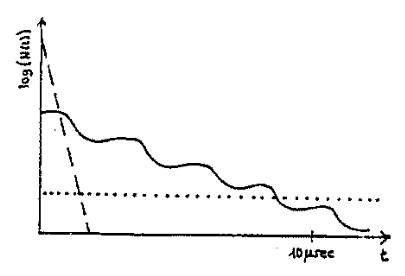
\includegraphics[width=\linewidth]{./fig/wigl1.png}
  \caption{}
\label{sfig:wigl1}
  \end{subfigure}
   \begin{subfigure}[t]{0.49\linewidth}
  \centering
   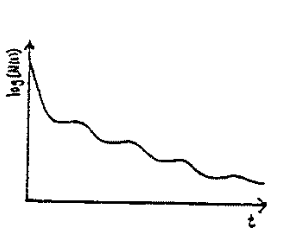
\includegraphics[width=\linewidth]{./fig/wigl2.png}
  \caption{}
\label{sfig:wigl2}
  \end{subfigure}
\caption{(a) Components of the expected decay spectrum. The stripped line represents the negative muons, the solid line represents positive muons and the dotted line represents the constant background (b) Total decay (with greatly exagerated asymmetry).}
\label{fig:wigl}
\end{figure}

\item \textbf{The background}

Accidental coincidences contribute to create a constant background $N_{\text{U}}(t)=U$.

Thus, overall the following distribution is expected:

\begin{equation}
N(t)=N_{-}e^{\frac{-t}{\tau_{-}}}+N_{+}(1+A\cos{\omega_{\text{L}}t+\Phi})e^{\frac{-t}{\tau_{+}}}+U.
\end{equation}

There are therefore eight parameters to consider: $N_{-}$, $\tau_{-}$, $N_{+}$, $\tau_{+}$, A, $\omega$, $\Phi$, $U$.

\end{enumerate}

\section{Analysis methods}

Once the data has been acquired through the PC, it must be analyzed, this is done through fitting the parameters of the expected distribution to the data. Two ways to do so will be discussed here: the \textit{optical fit} and the $\chi^2$-minimization-based \textit{SEEK} Algorithm.

\subsection{Optical fit}

The optical fit is, as it name suggests, a fit made by eye. The measured data points are displayed on a graph and one can then enter parameter values that are believed to well describe the distribution. Since estimating the cosine function form the \APmuon decay spectrum is difficult, the asymmetry factor $A$ is set to zero (as if no B-field was set) for optical fits. After recording the calibration of the TDC, it might be necessary to calibrate the data accordingly. For this purpose, the number of channels (each channel corresponds to \SI{50}{\nano\second} by which the measured data points need to be shifted (towards lower values) needs to be recorded in the time calibration field. This method has obvious faults: it's minimization is purely optical and thus quite unreliable, this is why one uses an automated $\chi^2$ minimization fit.

\subsection{$\chi^2$ minimization fit}

The $\chi^2$ can be seen as a measure of the distance of data points to the expectation of the measurement and is defined by:

\begin{equation}
\chi^2=\sum_{i=1}^{n}\frac{(O_i-E_i)^2}{E_i},
\end{equation}

where $O$ is the observed data value and $E$ is the expected data value for the given parameters. Given that data points are fixed, it is possible to vary the fitted function parameters and check the $\chi^2$ at every step to ensure that it is being minimized. This can of course be done by hand, but effective minimization routines have been developed and are commonly used to perform such fits, minimizing parameters in succession to try to find the most effective set for a minimal $\chi^2$. In order to judge the effectiveness of the fitting, a figure $\overline{\chi^2}=\frac{\chi^2}{N_{\text{df}}}$ is commonly used, with $N_{\text{df}}$ the number of degrees of freedom. The number of degrees of freedom is defined by the number of independent sample points used to compute a statistic minus the number of parameters estimated from the sample points. A $\overline{\chi^2}\sim 1$ is the sign of a good fit, $\overline{\chi^2} < 1$, on the other hand, suggest overfitting: the overestimation of degrees of freedom.


One should also be careful not to let the fitting engine get stuck in a local minimum of the $\chi^2$ distribution by using different starting values for the fit.

Popular $\chi^2$ fitting engines in high energy physics are CERN ROOT's MINUIT algorithm \cite{MINUIT} which can easily be used through a \texttt{TF1} fit or Python's scipy's \texttt{optimize.curve\_fit} and 

\texttt{optimize.leastsq} which both make use of the Levenburg-Marquardt gradiant method \cite{article}.

